% AEJ-Article.tex for AEA last revised 22 June 2011
\documentclass[AEJ,reviewmode]{AEA}

% The mathtime package uses a Times font instead of Computer Modern.
% Uncomment the line below if you wish to use the mathtime package:
%\usepackage[cmbold]{mathtime}
% Note that miktex, by default, configures the mathtime package to use commercial fonts
% which you may not have. If you would like to use mathtime but you are seeing error
% messages about missing fonts (mtex.pfb, mtsy.pfb, or rmtmi.pfb) then please see
% the technical support document at http://www.aeaweb.org/templates/technical_support.pdf
% for instructions on fixing this problem.

% Note: you may use either harvard or natbib (but not both) to provide a wider
% variety of citation commands than latex supports natively. See below.

% Uncomment the next line to use the natbib package with bibtex
\usepackage{natbib}
\usepackage{multirow}
\usepackage{graphicx}
\usepackage{tabularx}
\usepackage{microtype}

% Uncomment the next line to use the harvard package with bibtex
%\usepackage[abbr]{harvard}

% This command determines the leading (vertical space between lines) in draft mode
% with 1.5 corresponding to "double" spacing.
\draftSpacing{1.5}

\begin{document}

\title{A World Without Borders Revisited: The Impact of Online Sales Tax Collection on Shopping and Search}
\shortTitle{Online Shopping and Sales Tax}
\author{Mallick Hossain\thanks{%
Federal Reserve Bank of Philadelphia, Ten Independence Mall, Philadelphia, PA, 19106, mallick.hossain@phil.frb.org. The views expressed here are those of the author and do not necessarily represent the views of the Federal Reserve Bank of Philadelphia or the Federal Reserve System. I wish to thank Frank DiTraglia and Katja Seim for their advice and constructive criticism. Thanks also to Emek Basker, Ian Fillmore, Vitoria Rabello de Castro, and the participants of the Economic Graduate Student Conference at Washington University in St. Louis, the University of Pennsylvania Empirical Microeconomics Lunch, and the Empirical Microeconomics Student Workshop for their comments. Wharton Research Data Services (WRDS) was used in preparing this article. This service and the data available thereon constitute valuable intellectual property and trade secrets of WRDS and/or its third-party suppliers. Researcher's own analyses calculated based in part on data from The Nielsen Company (US), LLC and marketing databases provided through the Nielsen Datasets at the Kilts Center for Marketing Data Center at The University of Chicago Booth School of Business. The title is a reference to Goolsbee's 2000 paper that first examined the relationship between online shopping and sales taxes.}}
\date{\today}
\pubMonth{Month}
\pubYear{Year}
\pubVolume{Vol}
\pubIssue{Issue}
\JEL{D12, H31, H71, L81, M38}
\Keywords{sales tax, online shopping, e-commerce, Amazon, retail}

\begin{abstract}
I study the effect of closing the online sales tax loophole on online spending and search. Using online shopping data, sales taxes, and Amazon's staggered sales tax collection, I estimate that household price elasticity is $-$1.9, implying a 13\% decline in Amazon's revenues upon sales tax collection. After Amazon collects sales taxes, households increase their spending on Amazon's taxed competitors, but not its untaxed competitors. I find no evidence that households change their browsing or shift their spending offline. Collecting sales taxes online will help governments recapture lost taxes and increase online competition, but will not shift customers back offline.
\end{abstract}

\maketitle

Online shopping has grown dramatically since 2000, reaching 11.8\% of total retail sales in Q1 of 2020 \citep{CensusECom}. Reasons for this growth include lower costs (travel, time, etc.), higher convenience, and more variety \citep{forbes2013, powerRetail}. Until 2018, purely online retailers did not have to collect sales tax on online purchases because of a loophole in sales tax laws. As a result, purely online retailers could offer consumers, on average, a 7\% discount compared to brick-and-mortar retailers, a large, structural price advantage. This discount came strictly at the expense of state and local tax revenues, with losses ranging from \$8 to \$33 billion in 2018 \citep{wayfair2018}.

In this paper, I estimate consumers' price elasticity using price increases generated by sales taxes on online purchases. Due to pressure from state and local governments and aggressive fulfillment center expansion, online retailers (particularly Amazon) collect sales taxes in many states. Combining data on online shopping with local tax rates and Amazon's tax collection behavior across states over time, I estimate how consumers' online purchasing changes when sales taxes are collected online. Furthermore, I extend this analysis to include measures of online browsing as well as overall household spending (including offline expenditures) to estimate whether consumers' search behavior or their composition of online and offline spending changes in response to online sales tax collection.

I merge online shopping data with offline sales tax rates to estimate whether areas with higher tax rates respond more strongly to Amazon's sales tax collection. Previous research uses a variety of approaches to determine how sensitive consumers are to tax rates. Table \ref{tab:elasticity} summarizes elasticity estimates from previous research. In the offline environment, research leverages cross-border variation in tax rates and estimates a wide range of elasticities from $-30$ to $-0.2$ \citep{asplundFribergWilander2007, agarwal2017b, davis2011, agarwal2017a, mikesell1970}. In the online environment, elasticity estimates range from $-6$ to 0, but early efforts often used data from before 2001, i.e., before the mass adoption of the internet and before groundbreaking innovations like rating systems and free shipping were effectively implemented \citep{scanlan2007, ballardLee2007, almMelnik2005, goolsbee2000}. Recent work leverages detailed online shopping data, but often is limited to particular websites, product categories, or states \citep{einavEtAl2014, Anderson2010, Ellison2009, Hu201484}. My paper extends the work of \citet{baughBenDavidPark2016} and \citet{houdeNewberrySeim2016} by incorporating data on browsing and total household expenditures to present a fuller picture of how household shopping behavior changes in response to Amazon's sales tax collection.

\begin{table}
\centering
\caption{Estimated Elasticities}
\label{tab:elasticity}
\begin{tabular}{lll}
\hline
\textbf{Elasticity Type}           & \textbf{Paper}                     & \textbf{Estimate}     \\
\hline \hline
\multirow{6}{3.5cm}{\textbf{Cross-border Price-Expenditure}} &
  Asplund et al. (2007) -- Foreign price    & 0.2 to 0.5   \\
& Asplund et al. (2007) -- Domestic price & -0.2 to -1.3 \\
& Agarwal et al. (2017)                 & -2 to -30    \\
& Davis (2011)                                        & -2.2 to -3.6 \\
& Agarwal et al. (2017)            & -2.3         \\
& Mikesell (1970)                                     & -6.3         \\ \hline
\multirow{5}{3.5cm}{\textbf{Tax-Purchase}} &
  Scanlan (2007)                                        &  0.0          \\
& Ballard and Lee (2007)                               & -0.2          \\
& Alm and Melnik (2005)                                & -0.5          \\
& Einav et al. (2014)        & -1.8          \\
& Goolsbee (2000)                                     & -2.3          \\ \hline
\multirow{2}{3.5cm}{\textbf{Tax-Quantity}} &
  Anderson et al. (2010)          & -1.9 to -2.9  \\
& Ellison \& Ellison (2009)                           & -6            \\ \hline
\multirow{3}{3.5cm}{\textbf{Tax-Expenditure}} &
  Baugh et al. (2018)                      & -1.2 to -1.4  \\
& Houde et al. (2017)                     & -1.3          \\
& Hu and Tang (2014)                                  & -3.75 to -4.5 \\ \hline
\end{tabular}
\begin{tablenotes}
Early research focused on how taxes influenced the binary decision of whether or not to make an online purchase. Subsequent research has looked at how sales taxes affect actual online expenditures or quantities purchased. In order to distinguish between these concepts, I use ``tax-purchase elasticity'' to refer to the effect on the purchase decision while ``tax-quantity elasticity'' and ``tax-expenditure elasticity'' refer to the effect on online purchase quantities and expenditures, respectively.
\end{tablenotes}
\begin{tablenotes}[Source]
Sources are the papers cited above.
\end{tablenotes}
\end{table}


I use a differences-in-differences approach to estimate a household's price elasticity. The expansion of Amazon's warehouse network and the passage of state laws requiring online sales tax collection generate variation in Amazon's tax liability across states over time. As a result, I can examine how household behavior changes after Amazon collects sales taxes. Furthermore, I leverage variation in tax rates between counties to better examine if a household's responsiveness depends on their local tax rate.

I find that consumers reduce their Amazon spending by about 1.9\% for each percentage point of sales tax applied online. Given an average sales tax rate of 7\%, this elasticity translates into a 13\% decline in retail spending on Amazon. Consumers also increase their spending on Amazon's taxed competitors by 1\% per percentage point of sales tax collected by Amazon. This is one of the first papers to explicitly incorporate how consumer search behavior changes in response to tax changes. Even though consumers do shift their spending from Amazon to its competitors, I find no evidence that consumers' browsing habits are significantly affected by Amazon's sales tax collection. This is also one of the first papers to examine whether households shift their spending offline in response to online sales tax collection. I find no evidence that consumers make such a shift.

These findings show that state-level tax policy achieves its goals of increasing tax revenues and improving competition, but not necessarily of supporting local brick-and-mortar retailers. First, since consumers only shift spending between taxed online retailers, states and localities recover tax revenues that had disappeared when consumers made online purchases. At the same time, these policies restore competition between online retailers by removing the structural price advantage online retailers could pass on to customers. Finally, I find no evidence that consumers shift any spending back offline so these policies are unlikely to provide a boost for local brick-and-mortar retailers.

This paper is organized as follows. Section \ref{sec:data} describes the data. Section \ref{sec:model} analyzes how online spending responds to Amazon sales tax collection. Section \ref{sec:browse} examines whether online browsing activity is affected by Amazon sales tax collection. Section \ref{sec:nielsen} analyzes tax responsiveness across all consumer spending modes and Section \ref{sec:conclusion} concludes.

\section{Data Description}
\label{sec:data}

In this section, I describe the data used for my analysis and give a brief overview of their respective features.\footnote{Researcher's own analyses derived based in part on data from The Nielsen Company (US), LLC and marketing databases provided through the Nielsen Datasets at the Kilts Center for Marketing Data Center at The University of Chicago Booth School of Business.} Comscore's Web Behavior database provides information on household online shopping and browsing behavior. Nielsen's Consumer Panel data provides information on household shopping and purchasing decisions. Finally, Tax Data Systems provides information on local sales tax rates.

\subsection{Comscore Web Behavior Database}
I primarily use the Comscore Web Behavior database, which contains the online browsing and transaction activity of households that opt-in to have their internet activity collected by Comscore. The browsing data records how many minutes were spent and how many pages were viewed on each website. The transaction data records the website, product name, product category, price, quantity, and basket total (including shipping and taxes) of the purchase. The Comscore data capture all online activity of a household and is not limited to particular goods or retailers, in contrast with previous research. I use this breadth of information to capture whether households substitute to other retailers and estimate how their aggregate online spending changes when sales taxes are collected online.

I restrict my sample to households that have complete demographic information and remove any purchases in categories which Amazon is a not competitor (e.g., no plane tickets, dating services, etc.) and focus on products that cost between \$1 and \$500 (in nominal dollars).\footnote{This restriction is primarily to screen out extreme prices that may be generated by the Comscore monitoring software. For example, a \$20 item reduced to \$15 may mistakenly be recorded as \$2015 because of how the price information is captured.} These filters reduce the original sample of about 576,000 households to about 206,000 households and a total of about 2 million transactions.

Comscore households are relatively representative of the U.S. population. The average household size is 3, average age is 47, and average income is \$59,000. About 64\% of the households have a child and 13\% are Hispanic. Households face an average sales tax rate of 7\%. Overall, panelists are similar to the general population, but are slightly larger and more likely to have kids. Households rotate through Comscore's panel with a median tenure of 12 months (the 25th percentile is 9 months and the 75th percentile is 12 months). See Appendix Table \ref{tab:comScorePanel} for full summary statistics.

Across the two million transactions I analyze, the average real price of products (in December 2016 dollars) is \$39. 28\% of products are purchased on Amazon, 42\% from the website of a brick-and-mortar store and the remaining products are purchased from another online retailer. For browsing behavior, the average household spends about two and a half hours per month on shopping websites. Browsing on Amazon's untaxed competitors accounts for about one and a half hours, browsing on Amazon accounts for about 20 minutes and the remaining 40 minutes is on Amazon's taxed competitors. There is a wide range of shopping behavior with many households spending no time on shopping websites in a given month and others spending up to five hours per day. See Appendix Tables \ref{tab:comScoreSummary} and \ref{tab:comScoreBrowsing} for shopping and browsing summary statistics.

\subsection{Nielsen Consumer Panel Data}
I use the Nielsen Consumer Panel data from 2004--2016. This is a panel of about 178,000 unique households. I observe about 40,000 households each year from 2004--2006 and about 60,000 households each year from 2007--2016. Households scan all items that they purchase and then input information about quantities, prices, date of purchase, and store. Nielsen retains about 80\% of its panel from year to year with the mean and median tenure of a household being four and three years, respectively.

Nielsen computes projection weights to ensure their sample is nationally representative. Weights are calculated to match population moments based on household size, income, age, race, ethnicity, education, occupation, and presence of children. All analyses use these projection weights unless otherwise stated. Full summary statistics are reported in Appendix Table \ref{tab:homescanSummaryStats}.

Unlike the Comscore data, store identities are anonymized, but they are classified into broad categories such as ``Grocery Stores,'' ``Electronics Store,'' and ``Online Shopping.'' This categorization is enough to conduct a similar analysis as I do with the Comscore data, with the caveat that the Nielsen data primarily focus on basic household goods, so items like electronics and apparel will not be captured. For retailers with both an online and offline presence, Nielsen classifies them separately. For example, if Firm X has both offline stores and a website, detergent purchased from a Company X store will be from a different ``retailer'' than detergent purchased from CompanyX.com. In the first case, the retailer would be classified as a ``Discount Store'' and in the second, the retailer is classified as ``Online Shopping.''

For my analysis, I exclude tobacco and alcohol products because state and federal laws regulate purchasing these products online. I also remove households with a student or military head of household as well as those with an annual income of less than \$5,000. Only about 2\% of households are excluded and I use the remaining 154,000 households for my analysis. See Appendix \ref{sec:sampleConstruction} for further details of sample construction.

\subsection{Additional Data Sources}
I obtain state, county, and local sales tax rates from Tax Data Systems, now part of Thomson Reuters. These data contain monthly tax rates at the ZIP code level. I manually compile information on state law changes and agreements with Amazon under which states began collecting taxes for online transactions. This information was gathered from a wide range of local, state, and national news sources. Prior to 2018, most states did not require online retailers to collect sales taxes. They have only been able to collect sales taxes from Amazon because of separate agreements or because Amazon opened warehouses in their state.\footnote{\textit{National Bellas Hess v. Illinois} (1967) and \textit{Quill Corp. v. North Dakota} (1992) ruled that retailers did not have to collect sales taxes in states where they did not have a physical presence. The Court held that tabulating tax liabilities for over 6,000 different tax jurisdictions would place an undue burden on many of these firms \citep{taxFound2005}. The Supreme Court overturned these cases in \textit{South Dakota v. Wayfair Inc.} (2018). Before 2018, consumers were supposed to self-report any unpaid taxes to the tax authorities, but compliance and enforcement were low, so these transactions were effectively tax-free \citep{manzi2015}.} Before 2006, Amazon only collected sales taxes in Kansas, Kentucky, North Dakota, and Washington. By the end of 2016, Amazon collected sales taxes in an additional 25 states: Alabama, Arizona, California, Colorado, Connecticut, Florida, Georgia, Illinois, Indiana, Maryland, Massachusetts, Michigan, Minnesota, Nevada, New Jersey, New York, North Carolina, Ohio, Pennsylvania, South Carolina, Tennessee, Texas, Virginia, West Virginia, and Wisconsin.

Figure \ref{fig:taxStats} shows the wide variation in sales tax rates across the United States in December 2016. About 80\% of counties have combined state and local sales tax rates between 5.3\% and 8.3\%. However, sales tax rates range from 0\% to over 10\% in Louisiana.

\begin{figure}
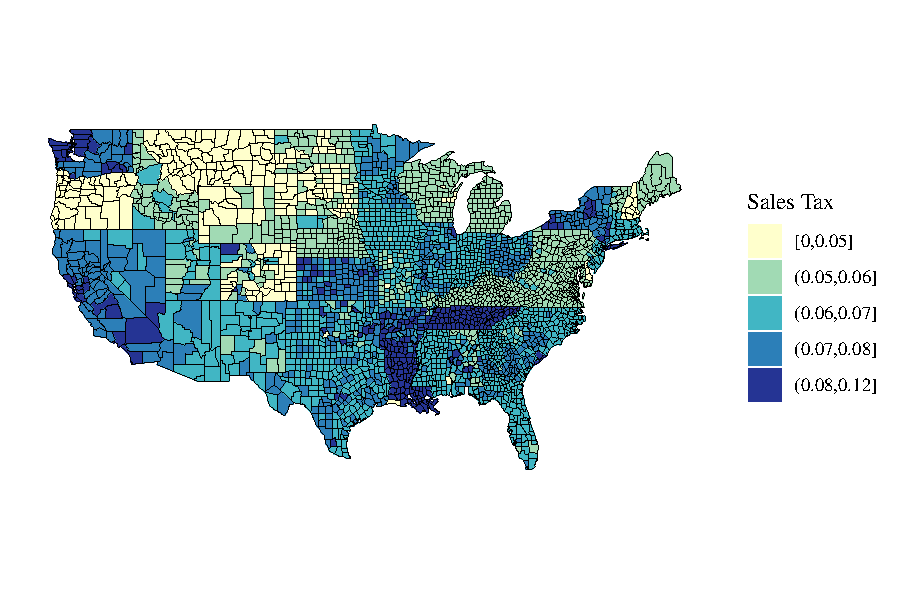
\includegraphics[width = 0.9\textwidth]{../5_figures/taxRateByCounty.pdf}
\caption{Sales Tax Rates by County (Dec 2016)}
\begin{figurenotes}
Figure plots the spatial distribution of sales tax rates.
\end{figurenotes}
\begin{figurenotes}[Source]
Tax Data Systems
\end{figurenotes}
\label{fig:taxStats}
\end{figure}

\section{Amazon Sales Tax Collection and Online Spending}
\label{sec:model}

When shopping online, households can purchase from Amazon or one of its competitors. Amazon has two types of competitors: taxed and untaxed. Amazon's taxed competitors consist of traditional brick-and-mortar retailers, like Walmart and Target, who collect sales tax since they have physical locations across the country. Amazon's untaxed competitors are other online retailers, like Overstock.com or Etsy.com, which do not have physical locations across the country (generally just a headquarters location).

When Amazon begins collecting sales tax, consumers could respond in a variety of ways. First, they may not change their behavior and continue purchasing purchase on Amazon (and maybe not even notice the sales tax). Second, they could switch to one of Amazon's competitors. They could switch to an untaxed competitor if they value the tax savings or possibly a taxed competitor that offers a better selection or lower tax-inclusive prices. I examine each of these in turn to see how spending on Amazon changes and how spending at Amazon's taxed and untaxed competitors changes after Amazon begins collecting sales taxes.

I use a differences-in-differences specification to identify the effect of Amazon's sales tax collection on a household's online spending:
\begin{equation}
\label{eq:model}
Y_{ht} = \alpha + \beta AmazonCollect_{ht} * \tau_{ht} + \lambda_h + \lambda_t + \epsilon_{ht},
\end{equation}
where $Y_{ht}$ measures real expenditures of household $h$ in month $t$. $AmazonCollect_{ht}$ indicates whether Amazon collects sales tax (determined by month and state of residence of the household). $\tau_{ht}$ is the local sales tax rate.\footnote{The local tax rate could also be included separately, but given the household fixed effect, this would only be identified off of changes in local tax rates which are relatively infrequent and when they do happen, are small.} Household and time fixed effects are captured by $\lambda_h$ and $\lambda_t$. $\beta$ is the coefficient of interest measuring how spending changes after Amazon begins collecting sales taxes relative to what would have been expected had they not started collecting sales taxes. All standard errors are clustered at the state level because once Amazon collects sales taxes, it collects them across the whole state.

The policy of whether or not Amazon collects sales tax in a particular state or county is plausibly exogenous to the household spending decision. Often, it is prompted by the opening of an Amazon warehouse in the state, but in a few cases, it is because of a change in state law. While there is a chance that these changes could be related to underlying economic fundamentals, \citet{baughBenDavidPark2016} show that sales tax collection by Amazon is not significantly related to state GDP growth, household income changes, or consumption declines. About 10\% of households experience a change in Amazon's sales tax collection while they are in the sample.


% Table created by stargazer v.5.2.2 by Marek Hlavac, Harvard University. E-mail: hlavac at fas.harvard.edu
% Date and time: Thu, Mar 12, 2020 - 04:21:17 PM
\begin{table}[!htbp] \centering
  \caption{Online Spending Response to Amazon Sales Tax Collection}
  \label{tab:spendingDiD}
\begin{tabularx}{\textwidth}{lXXXXXX}
\\[-1.8ex]\hline
\hline \\[-1.8ex]
 & Amazon & Untaxed Sites & Taxed Sites & Amazon & Untaxed Sites & Taxed Sites \\
\\[-1.8ex] & (1) & (2) & (3) & (4) & (5) & (6)\\
\hline \\[-1.8ex]
 Collect & $-$0.422 & $-$0.112 & 0.549 &  &  &  \\
  & (0.183) & (0.150) & (0.249) &  &  &  \\
  Collect * Tax Rate &  &  &  & $-$6.173 & $-$2.043 & 6.811 \\
  &  &  &  & (2.715) & (2.165) & (3.545) \\
 \hline \\[-1.8ex]
Household FE & Y & Y & Y & Y & Y & Y \\
Month-Year FE & Y & Y & Y & Y & Y & Y \\
Mean Spending & 3.30 & 4.86 & 7.01 & 3.30 & 4.86 & 7.01 \\
Mean Tax & 0.068 & 0.068 & 0.068 & 0.068 & 0.068 & 0.068 \\
Adjusted R$^{2}$ & 0.124 & 0.203 & 0.184 & 0.124 & 0.203 & 0.184 \\
Observations & \multicolumn{6}{c}{5,076,040} \\
\hline
\hline \\[-1.8ex]
\end{tabularx}
\begin{tablenotes}
This table reports the estimation results of Equation \ref{eq:model}, which regresses expenditures on an indicator for Amazon sales tax collection as well as household and month-year fixed effects. ``Collect'' is a dummy variable indicating whether Amazon collected sales tax in a particular household-month. ``Tax Rate'' measures the local sales tax rate faced by a household in a particular month. All expenditures are real expenditures, deflated to December 2016 using the CPI. ``Taxed Sites'' refers to websites of retailers that have offline stores. ``Untaxed Sites'' are online-only retailers with no offline stores. Standard errors are clustered at the state level.
\end{tablenotes}
\begin{tablenotes}[Source]
Comscore (2006--2016)
\end{tablenotes}
\end{table}


Table \ref{tab:spendingDiD} reports the estimation results. Columns (1) -- (3) only include an indicator for whether or not Amazon collects sales tax and then columns (4) -- (6) allow for the response to vary with the sales tax rate. Column (1) demonstrates that Amazon spending decreases by an average of \$0.422 after Amazon collects sales taxes. Given that average monthly spending on Amazon is \$3.30 and the average sales tax rate is 6.8\%, this equates to an elasticity of $\frac{-0.422 / 3.30}{0.068} = -1.88$. Columns (2) and (3) show that spending on Amazon's untaxed competitors does not significantly change while spending on its taxed competitors increases by \$0.549, implying a cross-elasticity of 1.14. Column (4) shows that the spending decreases on Amazon are stronger in areas with higher sales tax rates and the implied elasticity is a similar -1.87.\footnote{6.173 / 3.30 = -1.87} As before, there is no significant response on Amazon's untaxed competitors and a marginally significant increase on Amazon's taxed competitors. The spending increase on Amazon's taxed competitors implies an elasticity of 0.97. Overall, after Amazon collects sales taxes, households reduce their Amazon spending and increase their spending on Amazon's taxed competitors.

My estimated elasticity of $-1.88$ is higher (in magnitude) than similar estimates from \citet{baughBenDavidPark2016} and \citet{houdeNewberrySeim2016}. My estimate differs from \citet{houdeNewberrySeim2016} for two reasons. First, while I use the same underlying data, I extend my sample for another three years through 2016, which doubles the number of states in which Amazon begins collecting sales tax from 12 to 25. Second, their analysis aggregates the data to the county-year level, while I aggregate the data to the household-month level. I get nearly identical estimates if I aggregate to the county-year level and limit my sample to 2006--2013. My estimate also differs from \citet{baughBenDavidPark2016} likely because of differences in the underlying data. First, my analysis spans 2006--2016 compared to 2011--2015, which adds an additional six states to my analysis.\footnote{\citet{baughBenDavidPark2016} also restrict their analysis to households that spend more than \$200 on Amazon in 2011, but their Appendix B shows that removing this filter does not impact their estimate.} Restricting my analysis to 2011--2015 generates a slightly smaller elasticity of $-1.66$, but this is still higher than the $-1.2$ to $-1.4$ estimated in \citet{baughBenDavidPark2016}. The other possible contributor is the composition of our samples. The Comscore data captures all online activity on a household's computer and panelists are recruited to provide a representative measure of US internet users' activity. On the other hand, the data used in \citet{baughBenDavidPark2016} is from an online account aggregator that likely targets younger, tech-savvy users interested in managing their finances effectively.\footnote{One of the most popular financial aggregators, Mint.com, is reported to have a primarily young, male demographic. 71\% of users were male and 64\% were under 30 years of age back in 2008 \citep{perez2008}.} These users are probably more likely to shop online and may be less likely to switch away from Amazon. This assertion is supported by comparing the average monthly spending on Amazon between the two samples. The average monthly Amazon spending of a Comscore user is only \$3.30, but this increases to \$12.20 when restricting to only households that have made purchases on Amazon. In comparison, the average household in \citet{baughBenDavidPark2016} spends \$39. Overall, my estimate is higher than previous estimates because I incorporate more recent data and (arguably) a more representative sample of online shoppers.

\section{Amazon Sales Tax Collection and Online Browsing}
\label{sec:browse}

The previous section shows that consumers are spending less on Amazon and more on Amazon's taxed competitors. Do these changes in spending translate into changes in search behavior? I estimate Equation \ref{eq:model} with $Y$ being minutes spent on Amazon or one of its competitors' websites.


% Table created by stargazer v.5.2.2 by Marek Hlavac, Harvard University. E-mail: hlavac at fas.harvard.edu
% Date and time: Thu, Mar 12, 2020 - 10:08:26 PM
\begin{table}[!htbp] \centering
  \caption{Online Browsing Response to Amazon Sales Tax Collection}
  \label{tab:browsingDiD}
\begin{tabularx}{\textwidth}{lXXXXXX}
\\[-1.8ex]\hline
\hline \\[-1.8ex]
 & \multicolumn{6}{c}{Minutes Browsed} \\
\cline{2-7}
 & Amazon & Untaxed Sites & Taxed Sites & Amazon & Untaxed Sites & Taxed Sites \\
\\[-1.8ex] & (1) & (2) & (3) & (4) & (5) & (6)\\
\hline \\[-1.8ex]
 Collect & 0.076 & 0.387 & 0.512 &  &  &  \\
  & (0.435) & (0.977) & (0.640) &  &  &  \\
  Collect * Tax Rate &  &  &  & 0.369 & 6.317 & 7.160 \\
  &  &  &  & (5.695) & (12.840) & (9.243) \\
 \hline \\[-1.8ex]
Household FE & Y & Y & Y & Y & Y & Y \\
Month-Year FE & Y & Y & Y & Y & Y & Y \\
Mean Browsing (Min) & 11.71 & 66.66 & 27.98 & 11.71 & 66.66 & 27.98 \\
Mean Tax & 0.068 & 0.068 & 0.068 & 0.068 & 0.068 & 0.068 \\
Adjusted R$^{2}$ & 0.463 & 0.410 & 0.386 & 0.463 & 0.410 & 0.386 \\
Observations & \multicolumn{6}{c}{5,076,040} \\
\hline
\hline \\[-1.8ex]
\end{tabularx}
\begin{tablenotes}
This table reports the estimation results of Equation \ref{eq:model}, which regresses expenditures on an indicator for Amazon sales tax collection as well as household and month-year fixed effects. ``Collect'' is a dummy variable indicating whether Amazon collected sales tax in a particular household-month. ``Tax Rate'' measures the local sales tax rate faced by a household in a particular month. All browsing is in minutes. Standard errors are clustered at the state level.
\end{tablenotes}
\begin{tablenotes}[Source]
Comscore (2006--2016).
\end{tablenotes}
\end{table}


Table \ref{tab:browsingDiD} shows the results of this estimation. Our previous results indicate that households reduce their spending on Amazon only after sales tax is collected online. Because of this, we might expect that this reduced shopping activity would translate into reduced overall activity, measured in time spent on the website. Overall, I find no evidence that search on Amazon or its competitor websites is significantly affected by Amazon collecting sales tax. The lack of a significant browsing response may indicate that consumers are not changing their search behavior, but are simply switching their purchases away from Amazon since it no longer has a sales tax advantage.

Households' relative unresponsiveness in search effort contrasts with the findings of \citet{einavEtAl2014}, which finds that when buyers realize sales taxes are added, they back out of the transaction. This could be due to differences in user search between Amazon and eBay. On Amazon, the products are listed at a fixed price while on eBay, a share of items are sold at auction. In 2010 (the data used in \citet{einavEtAl2014}), 40\% of eBay sales were from auctions \citep{ebay2011}. Given the risk of losing the auction, customers may be more likely to search on eBay relative to Amazon, where there is no risk of losing the purchase. Even if there is an effect that I cannot detect, it is likely to be small changes in browsing time, which could be generated by the extra effort needed to complete the purchase (e.g., the time needed to enter in address and credit card information).

Overall, households reduce their pre-tax expenditures on Amazon and shift to Amazon's taxed competitors. In the next section, I examine whether households change their overall expenditures with a focus on whether their offline expenditures change in response to Amazon collecting sales tax.

\section{Total Consumer Expenditure Analysis}
\label{sec:nielsen}

The Comscore data suggest that consumers reduce their Amazon expenditures when Amazon begins collecting sales tax, but they do not spend or browse significantly more on Amazon's online competitors. The Comscore analysis is limited to examining only online transactions and activity. Using Nielsen's Consumer Panel Data, this section examines how households' overall spending changes in response to Amazon's sales tax collection. Households scan all of the items that they purchase for at-home consumption and input information about their shopping trip, including whether the purchase was from an online or offline retailer.\footnote{Retailers are anonymized in Nielsen, so I cannot identify whether an online purchase is made at a taxed or untaxed website as I could in the Comscore data.} Using these data, I can determine, for the common household items that are tracked, whether Amazon's sales tax collection changes overall household expenditures and whether households are shifting spending offline in response.

To identify changes in consumer expenditures, I estimate Equation \ref{eq:model} where $Y$ is the expenditures in either the online-only (likely untaxed) channel or offline channel. Since Amazon is most competitive in delivering less perishable, non-food products, I also separately examine whether online or offline non-food spending is affected. About 45\% of households experience a change in Amazon's sales tax collection during their tenure.


% Table created by stargazer v.5.2.2 by Marek Hlavac, Harvard University. E-mail: hlavac at fas.harvard.edu
% Date and time: Mon, Mar 16, 2020 - 01:38:47 AM
\begin{table}[!htbp] \centering
  \caption{Household Spending Response to Amazon Sales Tax Collection}
  \label{tab:nielsenDiD}
\begin{tabularx}{\textwidth}{lXXXXX}
\\[-1.8ex]\hline
\hline \\[-1.8ex]
 & \multicolumn{5}{c}{Real Spending} \\
\cline{2-6}
 & Total & Online & Offline & Online Non-Groc & Offline Non-Groc \\
\\[-1.8ex] & (1) & (2) & (3) & (4) & (5)\\
\hline \\[-1.8ex]
 Collect & $-$0.682 & 0.036 & $-$0.719 & 0.001 & 0.118 \\
  & (1.734) & (0.169) & (1.772) & (0.095) & (0.458) \\
 \hline \\[-1.8ex]
Household FE & Y & Y & Y & Y & Y \\
Month-Year FE & Y & Y & Y & Y & Y \\
Mean Spending & 316.39 & 4.7 & 311.69 & 2.93 & 94.74 \\
Mean Tax & 0.068 & 0.068 & 0.068 & 0.068 & 0.068 \\
Adjusted R$^{2}$ & 0.531 & 0.331 & 0.532 & 0.226 & 0.399 \\
Observations & \multicolumn{5}{c}{7,792,355} \\
\hline
\hline \\[-1.8ex]
\end{tabularx}
\begin{tablenotes}
This table reports the estimates from regressing monthly spending on an indicator for Amazon sales tax collection (``Collect'') as well as household and month-year fixed effects and household demographics. Standard errors are clustered at the state level.
\end{tablenotes}
\begin{tablenotes}[Source]
Nielsen Consumer Panel Data (2006--2016).
\end{tablenotes}
\end{table}


Table \ref{tab:nielsenDiD} shows that a range of household spending groups are unaffected by Amazon's sales tax collection. Columns (1) -- (3) show that there are no significant changes in total, online, or offline spending after Amazon begins collecting sales taxes. Even if there is an effect that I cannot detect, it is likely quite small. Part of this result is due to the fact that online shopping has low penetration into grocery and household non-durables (as indicated by monthly online spending averaging \$4). Even when analyzing only non-food items, where online shopping is most likely, there is no significant effect and the range of possible changes is quite small.

Because online shopping for household non-durables is relatively infrequent, the numerous months with no online expenditures may be masking changes in online purchases when they are made. This finding is robust to limiting the sample to  months when purchases are made (i.e. conditional on making a purchase). Overall, there is no evidence of households shifting their spending offline in response to Amazon's tax collection.

\section{Future Research and Conclusion}
\label{sec:conclusion}
Using data covering a broad range of online shopping activity, I find that consumers reduce their pre-tax spending on Amazon by about 1.9\% for every percentage point of sales tax that Amazon collects. Furthermore, I find that households increase their spending on Amazon's taxed competitors by 1\% for each percentage point of sales tax Amazon collects. Even though households change their spending, they do not significantly change their search behavior on Amazon or its competitors. Finally, I find no evidence that households shift any of their spending offline after Amazon collects sales tax.

In light of the recent Supreme Court case, \textit{South Dakota v. Wayfair} which increases state enforcement of sales tax collection online, state and local governments can expect a revenue boost because consumers are unlikely to shift their spending to untaxed channels. However, local policymakers and businesses will need to find other approaches if they want to encourage shoppers to move back offline. Online shopping is here to stay and more empirical work will be necessary to understand how offline retailers can adapt to increased online shopping.

% Bibliography
\bibliographystyle{aea}
\bibliography{reference}

% Appendix
\appendix

\section{Data Appendix}
\label{sec:sampleConstruction}

\subsection{Comscore Web Behavior}
This section provides more details about how I prepared the Comscore data for analysis. All Comscore data was obtained directly from Wharton Research Data Services (WRDS). I drop any households with incomplete demographic information. Additionally, I remove any households whose ZIP codes do not match with the Census Bureau's 2010 Zip-to-County Relationship file. Table \ref{tab:comScoreClean} shows that 35\% of households remain based on these filters. The low retention rate is primarily because a majority of Comscore households browse the internet and make no online purchases while they are in the sample. Table \ref{tab:comScorePanel} reports the summary statistics for the Comscore panel.


% Table created by stargazer v.5.2.2 by Marek Hlavac, Harvard University. E-mail: hlavac at fas.harvard.edu
% Date and time: Mon, Mar 09, 2020 - 01:17:40 PM
\begin{table}[!htbp] \centering
  \caption{comScore Sample}
  \label{tab:comScoreClean}
\begin{tabular}{@{\extracolsep{5pt}} cc}
\\[-1.8ex]\hline
\hline \\[-1.8ex]
Step & HH \\
\hline \\[-1.8ex]
Starting HH: & $586,420$ \\
Complete demographics: & $585,867$ \\
Valid ZIPs: & $576,457$ \\
Made Online Purchase: & $206,435$ \\
\hline \\[-1.8ex]
\end{tabular}
\begin{tablenotes}
Table reports the number of households remaining in sample after each step of data cleaning.
\end{tablenotes}
\end{table}



% Table created by stargazer v.5.2.2 by Marek Hlavac, Harvard University. E-mail: hlavac at fas.harvard.edu
% Date and time: Mon, Mar 09, 2020 - 03:20:55 PM
\begin{table}[!htbp] \centering
  \caption{comScore Panel Summary Statistics}
  \label{tab:comScorePanel}
\begin{tabular}{@{\extracolsep{5pt}}lccccc|c}
\\[-1.8ex]\hline
\hline \\[-1.8ex]
Statistic & \multicolumn{1}{c}{Mean} & \multicolumn{1}{c}{Median} & \multicolumn{1}{c}{St. Dev.} & \multicolumn{1}{c}{Min} & \multicolumn{1}{c}{Max} & Census (2016) \\
\hline
Household Size  & 3.04  & 3     & 1.40  & 1     & 6       & 2.53 \\
Age             & 46.65 & 47    & 12.59 & 19    & 65      & 51.9\\
Income          & 59.01 & 62.50 & 31.66 & 7.50  & 100.00  & 59.04 \\
Child Present   & 0.64  & 1     & 0.48  & 0     & 1       & 0.42 \\
Hispanic        & 0.13  & 0     & 0.34  & 0     & 1       & 0.13\\
Sales Tax       & 0.07  & 0.07  & 0.02  & 0.00  & 0.11    & - \\
\hline \\[-1.8ex]
N (Household-Years) & \multicolumn{6}{c}{261,416} \\
\hline \\[-1.8ex]
\end{tabular}
\caption*{Note: Age and income are reported in bins, so the midpoint of each bin is used. "Child Present" indicates whether a child is present in the household. Census data comes from "Historical Households Tables" and "Income and Poverty in the United States: 2016."}
\end{table}


For online transactions, I remove any transactions that are recorded for the same visit, same price, same time, and same product as a duplicate record. I also restrict my sample to products in categories that Amazon competes in, which excludes travel, dating, and financial products. Furthermore, I drop any transactions where the price is missing, less than \$1 or greater than \$500. Then, I remove any products that were sold by websites that do not feasibly compete with Amazon (e.g. daysinn.com or date.com).\footnote{The full list of domains is available in the replication code.} Table \ref{tab:transactionsClean} shows that most transactions are omitted because they are duplicates or in non-Amazon competitive categories. The remaining portion of transactions are removed because the household did not make any Amazon purchase while they were in the sample. Overall, 41\% of all transactions are made in Amazon competitive categories. Tables \ref{tab:comScoreSummary} and \ref{tab:comScoreBrowsing} report the summary statistics for online purchases and browsing in the Comscore data, respectively.


% Table created by stargazer v.5.2.2 by Marek Hlavac, Harvard University. E-mail: hlavac at fas.harvard.edu
% Date and time: Mon, Mar 09, 2020 - 04:55:17 PM
\begin{table}[!htbp] \centering
  \caption{comScore Transactions}
  \label{tab:transactionsClean}
\begin{tabular}{@{\extracolsep{5pt}} cc}
\\[-1.8ex]\hline
\hline \\[-1.8ex]
Step & Transactions \\
\hline \\[-1.8ex]
Starting Transactions: & $4,934,867$ \\
Unduplicated Transactions: & $3,956,424$ \\
Amazon Categories: & $2,478,115$ \\
Invalid Prices: & $2,269,680$ \\
Invalid Domains: & $2,021,800$ \\
\hline \\[-1.8ex]
\end{tabular}
\begin{tablenotes}
Table reports the number of transactions remaining in sample after each step of data cleaning.
\end{tablenotes}
\end{table}



% Table created by stargazer v.5.2.2 by Marek Hlavac, Harvard University. E-mail: hlavac at fas.harvard.edu
% Date and time: Mon, Mar 09, 2020 - 05:33:50 PM
\begin{table}[!htbp] \centering
  \caption{comScore Transaction Summary Statistics}
  \label{tab:comScoreSummary}
\begin{tabular}{@{\extracolsep{5pt}}lccccc}
\\[-1.8ex]\hline
\hline \\[-1.8ex]
Statistic & \multicolumn{1}{c}{Mean} & \multicolumn{1}{c}{Median} & \multicolumn{1}{c}{St. Dev.} & \multicolumn{1}{c}{Min} & \multicolumn{1}{c}{Max} \\
\hline \\[-1.8ex]
Real Product Price & 39.09 & 20.82 & 57.06 & 1.00 & 608.90 \\
Sales Tax & 0.07 & 0.07 & 0.02 & 0.00 & 0.11 \\
Amazon Purchase & 0.28 & 0 & 0.45 & 0 & 1 \\
Offline Amazon Competitor & 0.42 & 0 & 0.49 & 0 & 1 \\
Online Amazon Competitor & 0.30 & 0 & 0.46 & 0 & 1 \\
\hline \\[-1.8ex]
N & \multicolumn{1}{c}{2,001,485} \\
\hline \\[-1.8ex]
\end{tabular}
\begin{tablenotes}
Prices are deflated to December 2016 price levels using the CPI. ``Sales Tax'' indicates average local sales tax rate, not the average sales tax paid on online transactions.
\end{tablenotes}
\end{table}



% Table created by stargazer v.5.2.2 by Marek Hlavac, Harvard University. E-mail: hlavac at fas.harvard.edu
% Date and time: Sun, Mar 15, 2020 - 10:39:26 PM
\begin{table}[!htbp] \centering
  \caption{comScore Browsing Summary Statistics (Minutes)}
  \label{tab:comScoreBrowsing}
\begin{tabular}{@{\extracolsep{5pt}}lccccc}
\\[-1.8ex]\hline
\hline \\[-1.8ex]
Statistic & \multicolumn{1}{c}{Mean} & \multicolumn{1}{c}{Median} & \multicolumn{1}{c}{St. Dev.} & \multicolumn{1}{c}{Min} & \multicolumn{1}{c}{Max} \\
\hline \\[-1.8ex]
Total & 152.50 & 51.7 & 388.33 & 0 & 10,196 \\
Amazon & 18.52 & 0 & 83.19 & 0 & 8,864 \\
Untaxed Competitor & 93.46 & 16 & 346.00 & 0 & 10,176 \\
Taxed Competitor & 40.51 & 8 & 100.53 & 0 & 9,810 \\
\hline \\[-1.8ex]
N (Household-Months) & \multicolumn{4}{c}{2,559,012} \\
\hline \\[-1.8ex]
\end{tabular}
\begin{tablenotes}
Using 2006--2016 comScore Web Behavior data, this table reports the distribution of monthly browsing durations, in minutes, on shopping websites.
\end{tablenotes}
\end{table}


\subsection{Nielsen Consumer Panel Data}
This section provides more details about how I prepared the Nielsen Consumer Panel Data for analysis. I download the data directly from the University of Chicago Kilts Center for Marketing. I then remove any households with a military or student head of household or those that are making less than \$5,000 annually. Table \ref{tab:homeScanClean} shows that only 2\% of households are removed by these criteria. Table \ref{tab:homescanSummaryStats} reports the summary statistics for Nielsen households.


% Table created by stargazer v.5.2.2 by Marek Hlavac, Harvard University. E-mail: hlavac at fas.harvard.edu
% Date and time: Tue, Mar 10, 2020 - 02:57:06 PM
\begin{table}[!htbp] \centering 
  \caption{Homescan Sample} 
  \label{tab:homeScanClean} 
\begin{tabular}{@{\extracolsep{5pt}} cc} 
\\[-1.8ex]\hline 
\hline \\[-1.8ex] 
Step & HH \\ 
\hline \\[-1.8ex] 
Starting HH: & $158,004$ \\ 
Exclude military and students: & $155,256$ \\ 
Exclude Households under 5k: & $154,352$ \\ 
\hline \\[-1.8ex] 
\end{tabular} 
\end{table} 


\begin{table}[!htbp] \centering
\caption{Nielsen Consumer Panel Summary Statistics}
\label{tab:homescanSummaryStats}
\begin{tabular}{lcccc|c}
\\[-1.8ex]\hline
\hline
Variable                  & Mean  & SD    & 25th Pctile & 75th Pctile & Census (2016) \\
\hline
Household income (\$000s) & 56.53 & 31.41 & 27.5        & 85 & 59.04 \\
Household size            & 2.55  & 1.45  & 1           & 3  & 2.53 \\
Age                       & 52.62 & 14.34 & 41.5        & 63 & 51.9 \\
College Educated          & 0.38  & 0.48  & 0           & 1  & 0.37 \\
Child present             & 0.33  & 0.47  & 0           & 1  & 0.42 \\
Married                   & 0.50  & 0.50  & 0           & 1  & 0.48 \\
\hline
N (Household-Years)       & \multicolumn{4}{c}{637,493} \\
N (Households)            & \multicolumn{4}{c}{154,352} \\
\\[-1.8ex]\hline
\hline \\[-1.8ex]
\end{tabular}
\caption*{Note: Data are weighted for national representativeness.}
\end{table}


In the purchases data, I remove any alcohol and tobacco products as well as product categories that Nielsen has not consistently tracked over the full 2006--2016 period (i.e. ``deferred modules''). I also exclude products that do not have Universal Product Codes (i.e. ``magnet modules''). Finally, I remove any products with a recorded price of zero.

One final note for those familiar with Nielsen's data products. Theoretically, I could use the Scanner data to determine whether an ``online'' retailer and another retailer share the same parent company (for the set of retailers that Nielsen track in their data). Unfortunately, none of the ``Online Shopping'' retailer codes are present in the Nielsen Scanner Data, so I cannot distinguish if the online retailer is the website of a traditional brick-and-mortar store (and thus taxed) or a stand-alone online store (and thus untaxed).

\end{document}

% # Tax Law Appendix
% ## History
% In the late 1990's and early 2000's, widespread internet adoption and the growth of online retailers enabled households to make tax-free purchases. Often, websites would advertise that customers would pay no sales tax on purchases, often without mentioning that customers were responsible for remitting the unpaid sales tax.^[See \url{https://web.archive.org/web/20180525192327/https://shop.ccs.com/} for an example.]
%
% However, in 2008, New York passed a law that forced online retailers to collect sales taxes for shipments to New York residents. This began a cascade of other "Amazon Laws," some of which forced online retailers to collect sales taxes by broadening the definition of "physical presence." Most states claimed that if a retailer had an "affiliate" (e.g. a blogger paid to refer readers to the online retailer) in the state, that established a physical presence. However, in response, most online retailers (notably Amazon and Overstock) shut down their affiliate programs.
%
% Since then, some states have become more aggressive and require online retailers to either notify customers of their tax liability or to collect and remit the sales taxes themselves. These requirements cleverly sidestep the rulings of the Supreme Court and Colorado's effort to do this was upheld in court. Since then, online retailers have less aggressively challenged similar laws. As of April 1, 2017, Amazon collects state sales taxes in all 45 states that have state sales taxes and the District of Columbia. However, Amazon may not collect local sales taxes and these arrangements can differ by state.
%
% ## Sales Tax Heterogeneity
% The collection of sales taxes can differ within states due to state laws. First and foremost, some states do not collect sales taxes, others have a uniform sales tax state-wide, some allow counties to collect additional sales tax, but not cities, and others allow any locality (e.g. cities, special districts) to impose additional sales taxes. Furthermore, states can also decide whether they are an origin-based or destination-based sales tax state. In origin-based states, sales tax is collected based upon the location of the company selling the product. For example, Pennsylvania is an origin-based sales tax state, so Amazon does not collect the 2% Philadelphia county sales tax because its warehouse is not located in Philadelphia county. As a result, consumers in Philadelphia only pay 6% sales tax on Amazon versus 8% sales tax at brick-and-mortar retailers, but they still are responsible for remitting a 2% use tax to the county. Destination-based sales tax (which is more common) states require sales tax to be collected based upon the location of the buyer.
%
% ## Legislative Action
% There have been two main initiatives to improve sales tax collection from online retailers. Congressional action has taken the form of the Marketplace Fairness Act of 2017 (its previous incarnations were the Marketplace Fairness Act of 2011, 2013, and 2015). It was introduced in the Senate on April 27, 2017 and has been referred to committee. A more grassroots effort has been the Streamlined Sales Tax Project, started in 2000. This was created to help reduce the complexity in sales taxes that led to the _Bellas Hess v. Illinois_ and _Quill Corp. V. North Dakota_ decisions. By simplifying rules around sales tax, the hope is that complexity will no longer be a factor and there will be more fairness across the board (as well as higher revenues for states and localities). Currently, the project has 24 participating states that are working to create state-level administration of taxes, a uniform tax base, simplified tax rates, and uniform state sourcing rules.
%
% ## Timeline
%
% | Year       | States                                                     |
% |------------|------------------------------------------------------------|
% | 1995       | Washington                                                 |
% | 2001       | North Dakota                                               |
% | 2004       | Kansas                                                     |
% | 2005       | Kentucky                                                   |
% | 06/01/2008 | New York                                                   |
% | 07/01/2012 | Texas                                                      |
% | 09/01/2012 | Pennsylvania                                               |
% | 09/15/2012 | California                                                 |
% | 02/01/2013 | Arizona                                                    |
% | 07/01/2013 | New Jersey                                                 |
% | 09/01/2013 | Georgia, Virginia                                          |
% | 10/01/2013 | West Virginia                                              |
% | 11/01/2013 | Connecticut, Massachusetts, Wisconsin                      |
% | 01/01/2014 | Indiana, Nevada, Tennessee                                 |
% | 02/01/2014 | North Carolina                                             |
% | 05/01/2014 | Florida                                                    |
% | 10/01/2014 | Maryland, Minnesota                                        |
% | 02/01/2015 | Illinois                                                   |
% | 06/01/2015 | Ohio                                                       |
% | 10/01/2015 | Michigan                                                   |
% | 01/01/2016 | South Carolina                                             |
% | 02/01/2016 | Colorado                                                   |
% | 10/01/2016 | DC                                                         |
% | 11/01/2016 | Alabama                                                    |
% | 01/01/2017 | Iowa, Louisiana, Nebraska, Utah                            |
% | 02/01/2017 | Mississippi, Missouri, Rhode Island, South Dakota, Vermont |
% | 03/01/2017 | Arkansas, Oklahoma, Wyoming                                |
% | 04/01/2017 | New Mexico                                                 |
% Table: Timeline of Amazon Sales Tax Collections
%
% \newpage
%
% \begin{figure}[p]
%     \centering
%     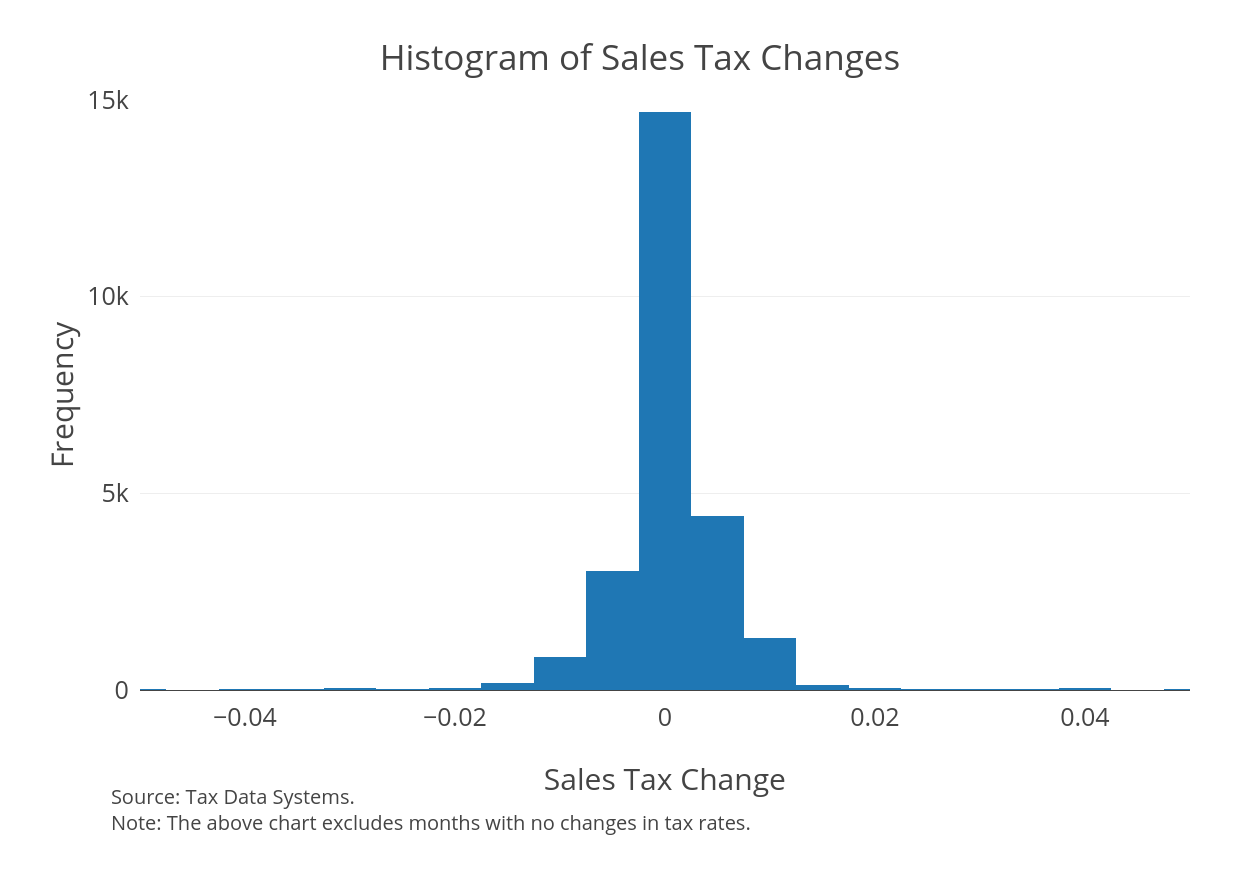
\includegraphics[width=\textwidth]{../5_figures/taxChangeHist.png}
%     \caption{}
%     \label{fig:taxChangeHist}
% \end{figure}
%
% \begin{figure}[p]
%     \centering
%     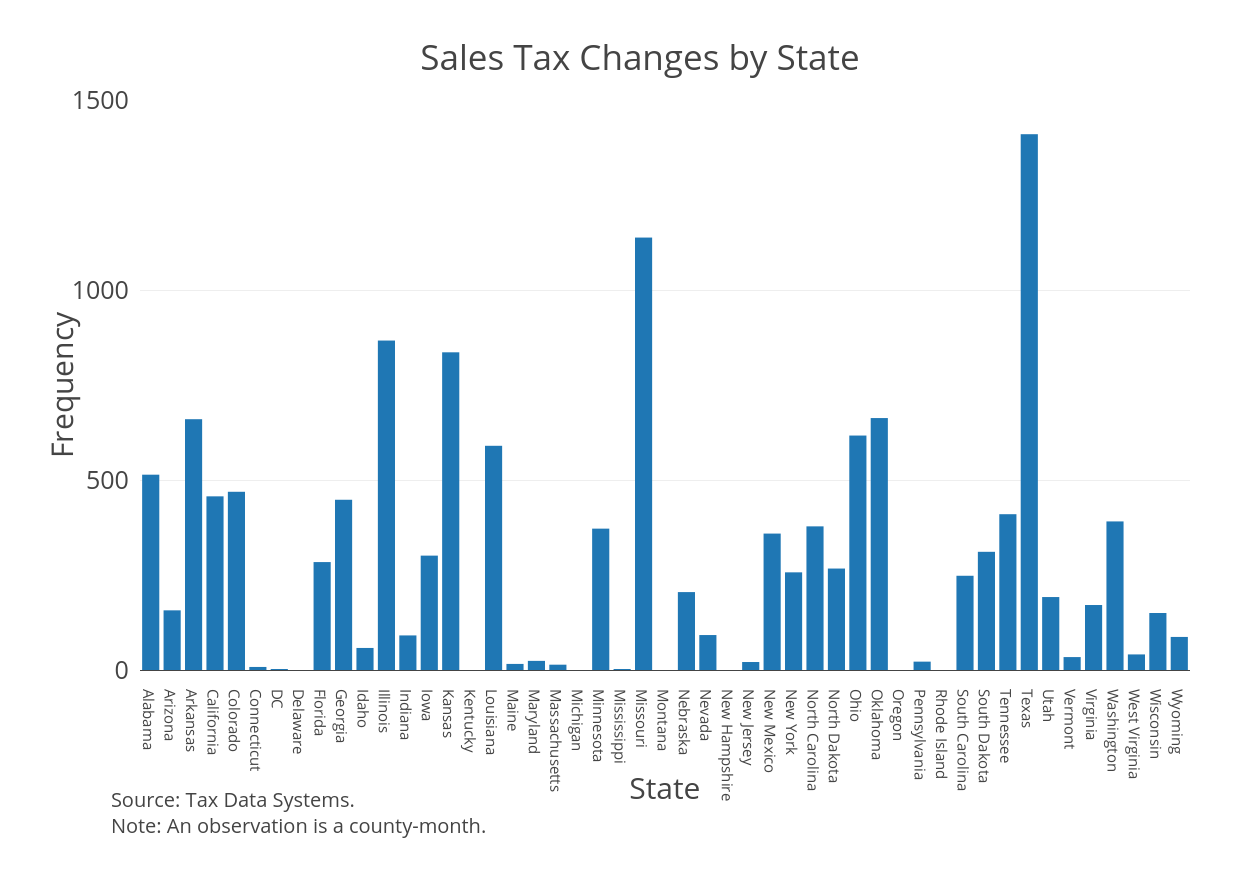
\includegraphics[width=\textwidth]{../5_figures/taxChangeByState.png}
%     \caption{}
%     \label{fig:taxChangeState}
% \end{figure}
%
% \begin{figure}[p]
%     \centering
%     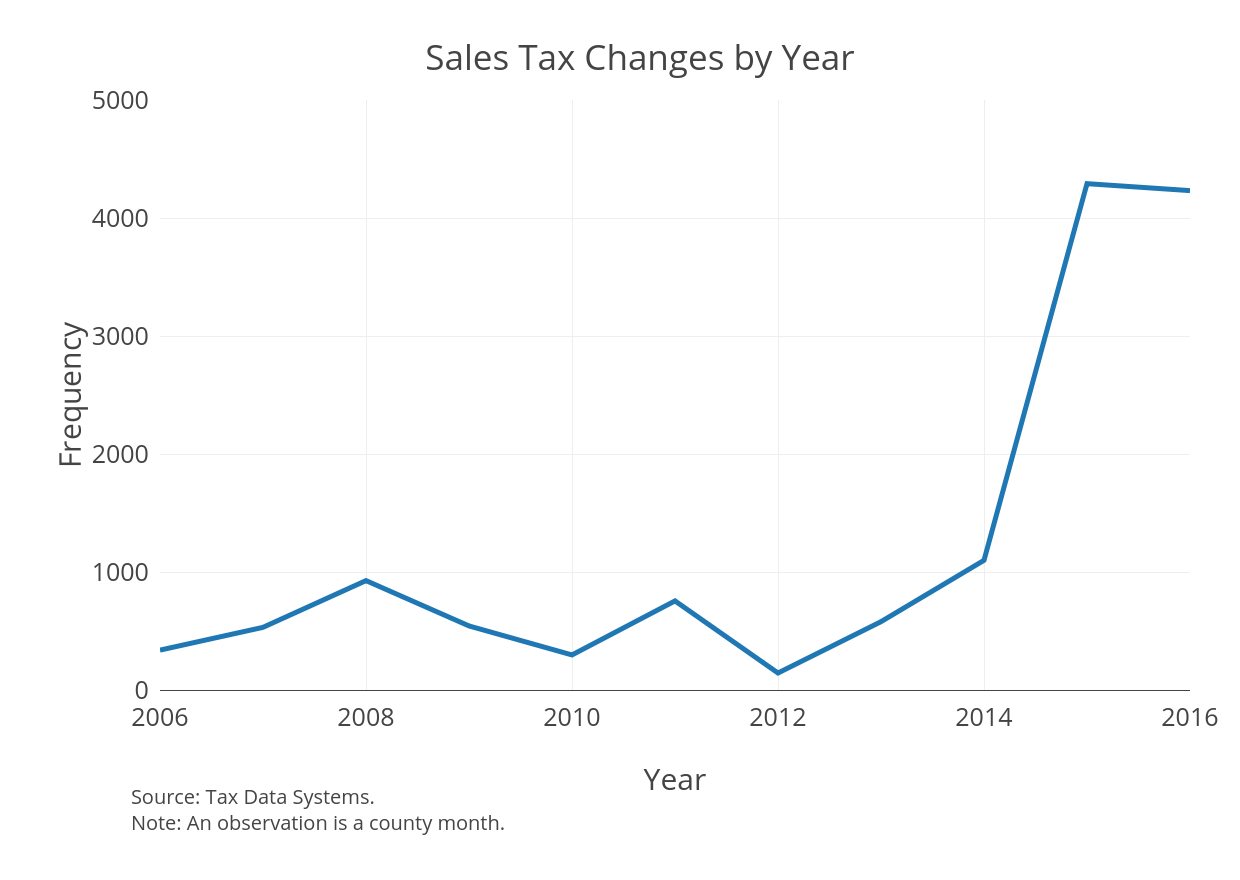
\includegraphics[width=\textwidth]{../5_figures/taxChangeByYear.png}
%     \caption{}
%     \label{fig:taxChangeYear}
% \end{figure}
